\documentclass[11pt, a4paper]{article}
\usepackage{graphicx}
\usepackage{amsmath}
\usepackage{listings}
\usepackage{minted}
\usepackage{physics}

\title{EE2703 Applied Programming Lab - Assignment No 8}
\author{
  \textbf{Name}: Atishay Ganesh\\
  \textbf{Roll Number}: EE17B155
}\date{\today}
\begin{document}
		
\maketitle 
\section{Abstract}
The goal of this assignment is the following.
\begin{itemize}
\item Obtaining the DFT of various functions.
\item To see how the DFT can be used to approximate the CTFT.
\item To plot graphs to understand this.
\end{itemize}
\usemintedstyle{manni}

\section{Assignment}
\subsection{Setting up the variables}
Importing the standard libraries
\begin{minted}[mathescape,escapeinside = ||]{python3}
from pylab import *
\end{minted}

\subsection{Inverting the FFT}
{
To verify that the fft and the ifft are inverses of each other, we call them and note the difference absolute max of the difference.
}
\begin{minted}{python3}
x=rand(100)
X=fft(x)
y=ifft(X)
c_[x,y]
print(abs(x-y).max())

\end{minted}
{
4.446383891599849e-16
The smalll error is due to numerical precision in taking the ifft.
There will be some imaginary part of the error again due to numerical precision.
}

\subsection{Calculating FFT, Trial 1}
{
We try to take the FFT of a sinusoid.
}
\begin{minted}{python3}

x=linspace(0,2*pi,128)
y=sin(5*x)
Y=fft(y)
figure()
subplot(2,1,1)
plot(abs(Y),lw=2) #line width of 2
ylabel(r"$|Y|$",size=16)
title(r"Spectrum of $\sin(5t)$")
grid(True)#for the grid
subplot(2,1,2)
plot(unwrap(angle(Y)),lw=2)
ylabel(r"Phase of $Y$",size=16)
xlabel(r"$k$",size=16)
grid(True)
savefig("fig8-1.png")#Automatically saving the figure
show()


\end{minted}
{
We get 2 peaks as expected but the peaks are in the wrong location and the scale of the x axis is wrong.
}
\begin{figure}[!tbh]
   	\centering
   	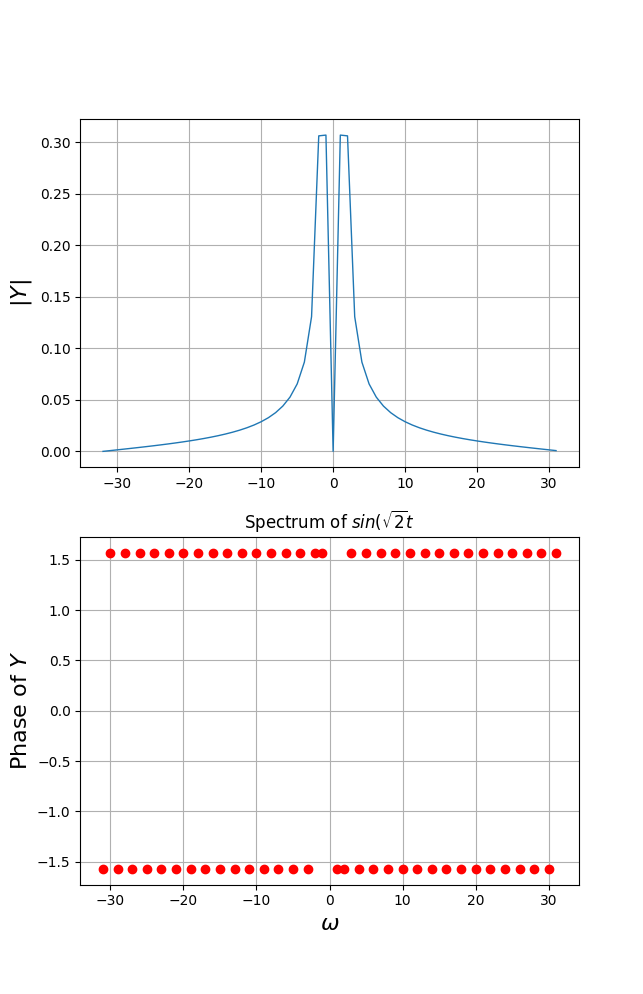
\includegraphics[scale=0.5]{fig9-1.png}
   	\label{fig:01}
   \end{figure}

\subsection{Calculating FFT, Trial 2} 
{
We try to take the FFT of a sinusoid,but now using fftshift() to correct the previous error. The error was due to the FFT being from 0 to 2*$\pi$ instead of -$\pi$ to $\pi$ as we would want. We also divide by the number of samples.
We also have to exclude the last sample as the DFT is a sampling of the DFT using evenly spaced samples.
}
\begin{minted}{python3}

x=linspace(0,2*pi,129);x=x[:-1]#so that last point is excluded
y=sin(5*x)
Y=fftshift(fft(y))/128.0#fftshift converts from [0,2pi] to [-pi,pi] 
w=linspace(-64,63,128)
figure()
subplot(2,1,1)
plot(w,abs(Y),lw=2)
xlim([-10,10])
ylabel(r"$|Y|$",size=16)
title(r"Spectrum of $\sin(5t)$")
grid(True)
subplot(2,1,2)
plot(w,angle(Y),'ro',lw=2)
ii=where(abs(Y)>1e-3)#highlighting points for which phase is relavant
plot(w[ii],angle(Y[ii]),'go',lw=2)
xlim([-10,10])
ylabel(r"Phase of $Y$",size=16)
xlabel(r"$k$",size=16)
grid(True)
savefig("fig9-2.png")
show()


\end{minted}
{
Finally it looks like what we expected with 2 peaks at the right frequencies.
}
\begin{figure}[!tbh]
   	\centering
   	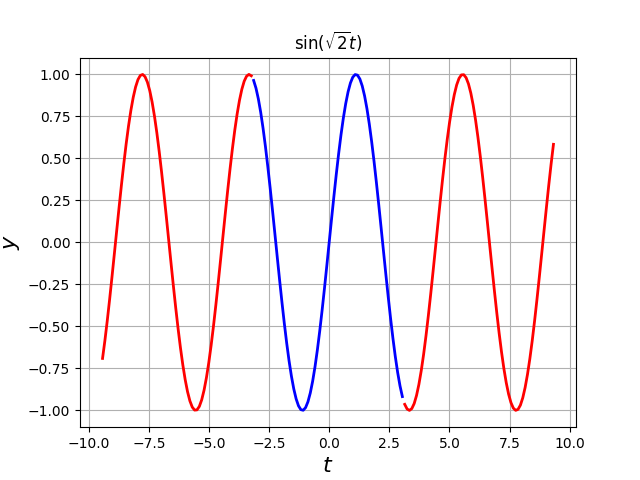
\includegraphics[scale=0.5]{fig9-2.png}
   	\label{fig:01}
   \end{figure}

\subsection{Calculating FFT, for AM} 
{
We try to take the FFT of an Amplitude Modulated Sinusoid of the form
$\left(1+0.1\cos\left(t\right)\right)\cos\left(10t\right)$
}
\begin{minted}{python3}
t=linspace(0,2*pi,129);t=t[:-1]#low sampling frequency,aliasing
y=(1+0.1*cos(t))*cos(10*t)#AM with carrier at 10 and modulating freq of 1
Y=fftshift(fft(y))/128.0
w=linspace(-64,63,128)
figure()
subplot(2,1,1)
plot(w,abs(Y),lw=2)
xlim([-15,15])
ylabel(r"$|Y|$",size=16)
title(r"Spectrum of $\left(1+0.1\cos\left(t\right)\right)\cos\left(10t\right)$")
grid(True)
subplot(2,1,2)
plot(w,angle(Y),'ro',lw=2)
xlim([-15,15])
ylabel(r"Phase of $Y$",size=16)
xlabel(r"$\omega$",size=16)
grid(True)
savefig("fig8-3.png")
show()


\end{minted}
{
Instead of getting 3 peaks, we only get 1 broad peak. This is because the number of samples are not sufficient to get the necessary information. This is known as aliasing.
}
\begin{figure}[!tbh]
   	\centering
   	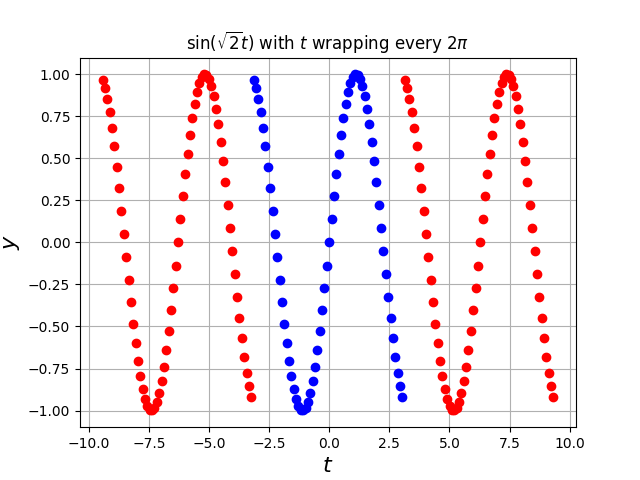
\includegraphics[scale=0.5]{fig9-3.png}
   	\label{fig:01}
   \end{figure}


\subsection{Calculating FFT, for AM, Trial 2} 
{
We increase the number of samples and try again.
}
\begin{minted}{python3}

t=linspace(-4*pi,4*pi,513);t=t[:-1]#higher sampling rate, no aliasing
y=(1+0.1*cos(t))*cos(10*t)
Y=fftshift(fft(y))/512.0
w=linspace(-64,64,513);w=w[:-1]
figure()
subplot(2,1,1)
plot(w,abs(Y),lw=2)
xlim([-15,15])
ylabel(r"$|Y|$",size=16)
title(r"Spectrum of $\left(1+0.1\cos\left(t\right)\right)\cos\left(10t\right)$")
grid(True)
subplot(2,1,2)
plot(w,angle(Y),'ro',lw=2)
xlim([-15,15])
ii=where(abs(Y)>1e-3)
plot(w[ii],angle(Y[ii]),'go',lw=2)
ylabel(r"Phase of $Y$",size=16)
xlabel(r"$\omega$",size=16)
grid(True)
savefig("fig8-4.png")
show()


\end{minted}
{
As expected, we get three peaks at the carrier band and at frequencies above and below the carrier band at frequency difference equal to the modulating frequency.
Most of the energy is stored in the carrier band.
}
\begin{figure}[!tbh]
   	\centering
   	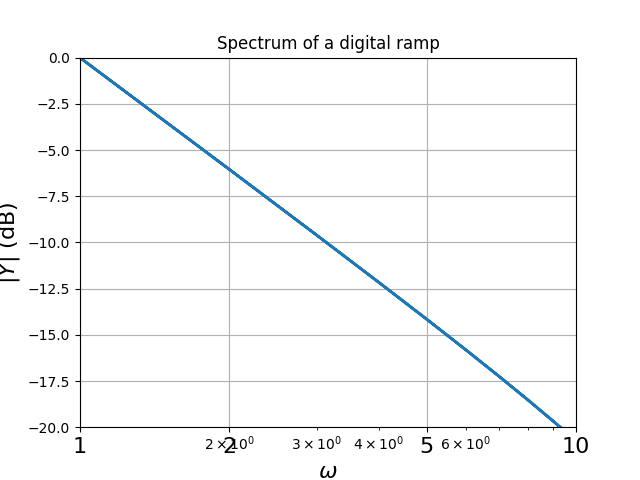
\includegraphics[scale=0.5]{fig9-4.png}
   	\label{fig:04}
   \end{figure}




\subsection{DFT Function}
{
We now create a function to plot the DFT (Using the FFT algorithm) for multiple different functions.
}
\begin{minted}{python3}


def dft(func,tim= None,n_p=512,fig_no=0,name= None):
'''Function to plot the dft using fft algorithm
func: lambda/function whose fourier transform is required
time: time interval in the form (start_time,end_time)
default is (-4*pi,4*pi)
n_p: number of samples in time domain
fig_no: Figure number
name: Name of function for the graph
'''
    if tim is None:
        t=linspace(-4*pi,4*pi,n_p,endpoint= False)
    else:
        start,end = tim
        t = linspace(start,end,n_p,endpoint=False)
    y = func(t)
    Y=fftshift(fft((y)))/n_p#fftshift so the plot is in terms we know
    w=linspace(-pi,pi,n_p,endpoint= False);
    w = w*n_p/(end-start)#the range of frequencies
    fig, (ax1, ax2) = plt.subplots(2, 1)
    Ysig = where(abs(Y)>10**-5)#only plot significant points phase
    ax1.plot(w,abs(Y),lw=1)
    ax1.set_xlim([-2*max(w[Ysig]),2*max(w[Ysig])])
    #to ensure that we dont go too far on each side

    ax1.set_ylabel(r"$|Y|$",size=16)
    title("Spectrum of {}".format(name))
    ax1.grid(True)
    ax2.plot(w[Ysig],angle(Y[Ysig]),'ro')
    ax2.set_xlim([-2*max(w[Ysig]),2*max(w[Ysig])])

    ax2.set_ylabel(r"Phase of $Y$",size=16)
    ax2.set_xlabel(r"$\omega$",size=16)
    grid(True)
    return ax1,ax2,w

\end{minted}


\subsection{FFT for $cos^{3}t$ and $sin^{3}t$}
{
We plot the DFT of the functions $cos^{3}t$ and $sin^{3}t$
below.
}
\begin{minted}{python3}
y1 = lambda t : (cos(t))**3
y2 = lambda t : (sin(t))**3
dft(y1,(-4*pi,4*pi),256,1,r'$cos^{3}t$')
dft(y2,(-2*pi,2*pi),256,2,r"$sin^{3}t$")
plt.show()
\end{minted}
\begin{figure}[!tbh]
   	\centering
   	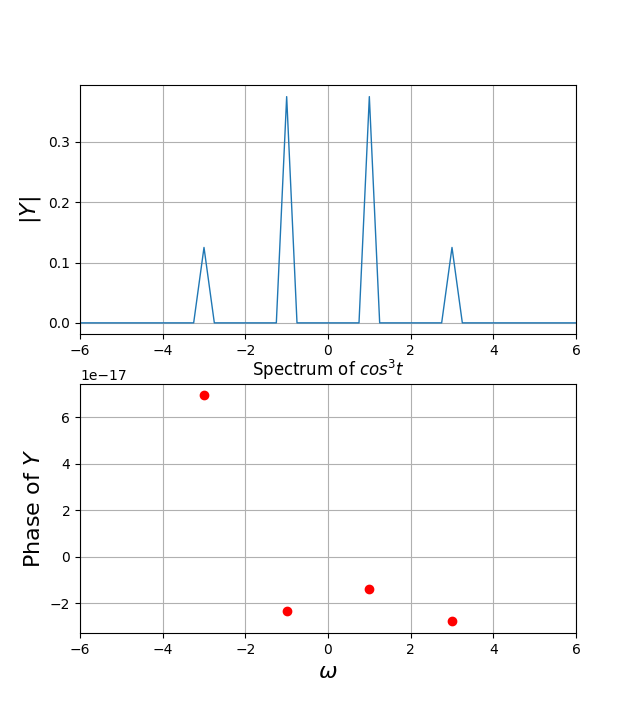
\includegraphics[scale=0.5]{img5.png}
   	\label{fig:32}
   \end{figure}
\begin{figure}[!tbh]
   	\centering
   	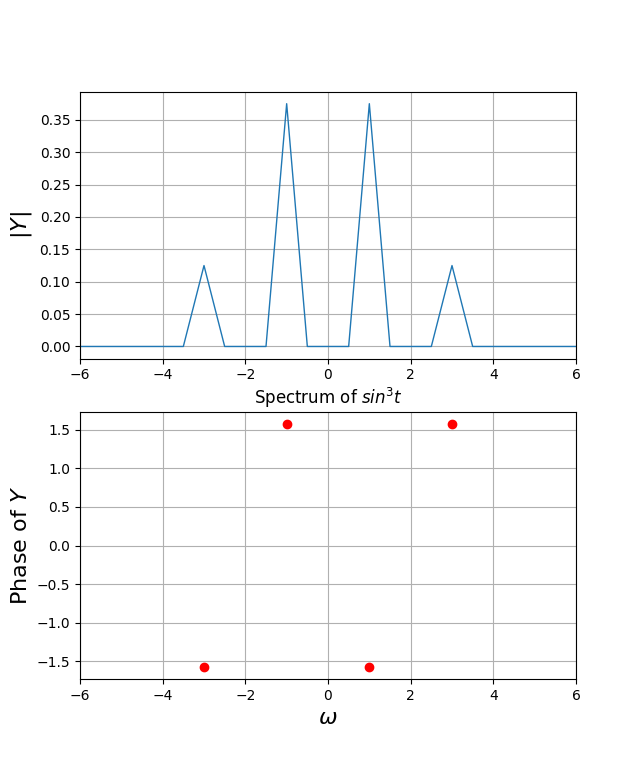
\includegraphics[scale=0.5]{img6.png}
   	\label{fig:32}
   \end{figure}
{
Both the spectrums have 4 peaks
These correspond to frequencies of $\pm$1 and $\pm$3. This is because
\[ \cos^3x =\frac{ \cos 3x +3\cos x}{4} \]
and
\[ \sin^3x =\frac{3\sin x-\sin 3x}{4} \]
Hence the peaks corresponding to $\pm$1 are thrice as big as the others.
}



\subsection{FFT for FM Sinusoid}
{
We plot the DFT of a frequency modulated sinusoid.
$\cos(20t+5\cos(t))$
}
\begin{minted}{python3}
y3 = lambda t : cos(20*t+5*cos(t))

dft(y3,(-4*pi,4*pi),2048,3,r"cos(20t+5cos(t))")

plt.show()
\end{minted}
\begin{figure}[!tbh]
   	\centering
   	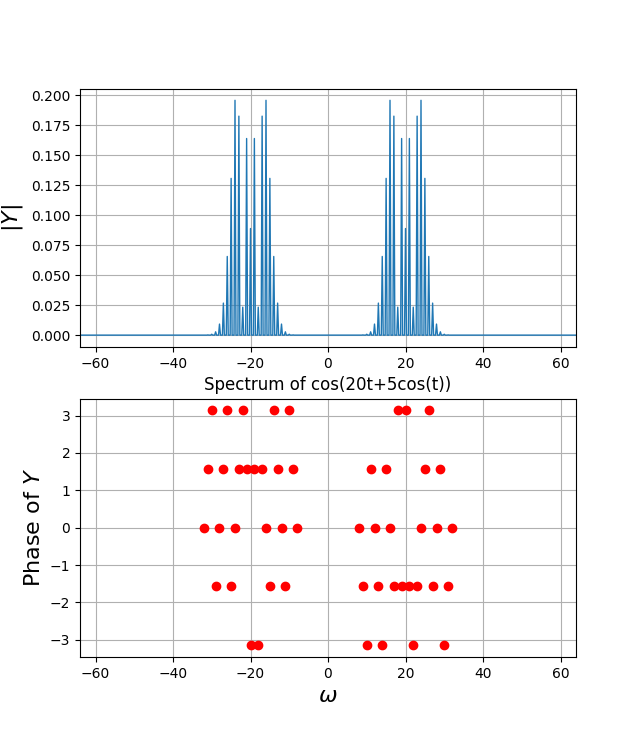
\includegraphics[scale=0.5]{img7.png}
   	\label{fig:32}
   \end{figure}
{
A lot of frequencies around the carrier band are present.
Most energy is carried by these.
}


\subsection{FFT for Gaussian}
{
We use the FFT to estimate the CTFT of the Gaussian distribution function
$e^{\frac{-t^2}{2}}$
\\
The CTFT of the above nonperiodic function is
$\frac{e^{\frac{-t^2}{2}}}{\sqrt{2\pi}}$,
using the appropriate CTFT Formulation.
}
\begin{minted}{python3}

def estctft(func,truth,tim= None,n_p=512,fig_no=0,name= None,):
'''Function to plot the dft using fft algorithm
func: lambda/function whose fourier transform is desired
truth: analytic ctft function/lambda
tim: time interval in the form (start_time,end_time)
default is (-4*pi,4*pi)
n_p: number of samples in time domain
fig_no: Figure number
name: Name of function for the graph
'''
    
    if tim is None:
        start=-4*pi
        end=4*pi
    else:
        start,end = tim

    t = linspace(end,start,n_p,endpoint=False)
    y = func(t)
    #ifftshift needed to remove certain phase issues
    Y=fftshift(fft(ifftshift(y)))*(end-start)/(2*pi*n_p)

    w=linspace(-pi,pi,n_p,endpoint= False);
    w = w*n_p/(end-start)
    
    #sum of total difference between the two transforms
    error = sum(abs(truth(w)-Y))
    print(error)
    #2.2822972865535313e-14
    fig, (ax1, ax2) = plt.subplots(2, 1)
    Ysig = where(abs(Y)>10**-5)
    ax1.plot(w,abs(Y),lw=1)
    ax1.set_xlim([-2*max(w[Ysig]),2*max(w[Ysig])])

    ax1.set_ylabel(r"$|Y|$",size=16)
    title("Spectrum of {}".format(name))
    ax1.grid(True)
    ax2.plot(w[Ysig],angle(Y[Ysig]),'ro')
    ax2.set_xlim([-2*max(w[Ysig]),2*max(w[Ysig])])
    #Only plot significant phase points
    ax2.set_ylabel(r"Phase of $Y$",size=16)
    ax2.set_xlabel(r"$\omega$",size=16)
    grid(True)
    return ax1,ax2,w

y4 = lambda t : exp(t**2/-2)
y5 = lambda w : exp(-w**2/2)/sqrt(2*pi)
start = 4*pi
#plot the true CTFT gotten analytically
ax1,ax2,w = estctft(y4,y5,(-start,start),1024,4,r"$exp(-t^{2}/2)$")

ax1.plot(w,abs(y5(w)),'y-')
ax2.plot(w,angle(y5(w)),'yo')
show()

\end{minted}


\begin{figure}[!tbh]
   	\centering
   	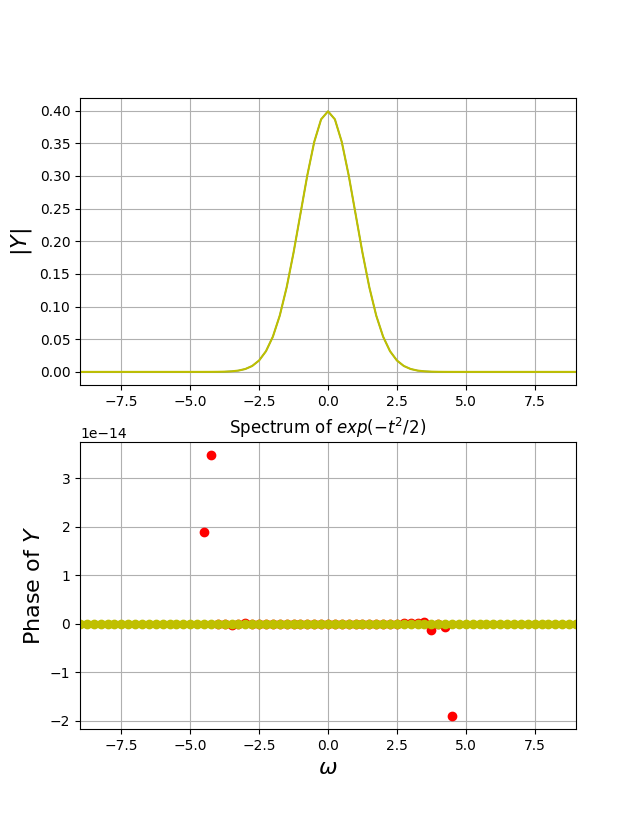
\includegraphics[scale=0.5]{img8.png}
   	\label{fig:32}
   \end{figure}
{
The error was
2.2822972865535313e-14
The error is almost negligible, and can easily be further reduced if necessary.
which  indicates the
IFFTShift was used to remove certain issues with the time domain form of the Gaussian
Phase is basically zero (within numerical precision), indicating the CTFT of the Gaussian is real valued and positive for all $\omega$. In fact, by observation we can say that it is also another Gaussian with same mean and standard deviation.
Thus it is clear that the Gaussian is the Eigenfunction of the Fourier Transform. 
}




\section{Conclusions}
\begin{itemize}
\item We analysed specta in the frequency domain using FFT.
\item We saw how the FFT can be used to emulate the CTFT.
\item We plotted graphs to understand the above.
\end{itemize}

\end{document}